\chapter{Probability}

\section{Basic concepts and results}

A \textbf{random experiment} is when a set of all possible outcomes is known, but it is impossible to predict the actual outcome of the experiment.
A \textbf{sample space}, denoted as $\Omega$, contains all possible outcomes of the experiment.
An \textbf{event} is a subset of $\Omega$. We say that $A\subset\Omega$ has occrred if and only if the outcome of the experiment is an element of $A$. 
Formally, the family of events forms a $\sigma$-algebra of subsets of $\Omega$ that we denote by $\mcA$.
\nt{
    \begin{itemize}
        \item $\Omega\in\mcA$
        \item $A\in\mcA\Rightarrow\bar{A}\in\bar{\mcA}$ ,where $\bar{A}$ indicates the compliment of A
        \item $A_1, A_2,\cdots\in\mcA$
        \item $\displaystyle\bigcup_{i=1}^{\infty}A_i\in\mcA$
    \end{itemize}
}
\subsection{Probability measures}
\dfn[]{Kolmogorov's axioms}{
    \begin{itemize}
        \item $P(A)\geq 0$
        \item $P(\Omega)=1$
        \item If $A_i\bigcap A_j = \emptyset, i\neq j$, then $P(\cup_i A_i) = \sum_i P(A_i)$
    \end{itemize}
}

Probability measure $P: \mcA\to\bbR$ satisfying Kolmogorov's axioms has the following properties:
\begin{itemize}
    \item $P(\varnothing) = 0$
    \item $A\subset B\Rightarrow P(A) \leq P(B)$
    \item $0\leq P(A)\leq 1$
    \item $P(A\cup B) = P(A) + P(B) - P(A\cap B)$
    \item $P(\bar{A}) = 1 - P(A)$
    \item $P(A-B) = P(A\cap \bar{B}) = P(A) - P(A\cap B)$
\end{itemize}

\dfn[]{Conditional probability}{
    If $P(B) > 0$,\\

    $\displaystyle P(A|B)=\frac{P(A\cap B)}{P(B)}$\\

    We are re-evaluating the probability of A given the B space.
}\bigskip

Let $\{A_1, A_2,\cdots\}$ denote a partition of $\Omega: \cup_i A_i = \Omega$; $A_i\cap A_j = \emptyset, i\neq j$.
Meaning union makes up $\Omega$ and are mutually exclusive. Then if $P(A_i)>0$ for all $i$
\thm[]{Total probability theorem}{
    $P(B) = \displaystyle \sum_i P(B|A_i)P(A_i)$
}
$B = B\cap \Omega = B\cap [\cup_i A_i] = \cup_i (B\cap A_i)$ and $P(\cup_i B\cap A_i) = \sum_i P(B\cap A_i)$
\thm[]{Bayes' theorem}{
    If $P(B)>0$\\

    $\displaystyle P(A_i|B) = \frac{P(B|A_j)P(A_j)}{\sum_i P(B|A_i)P(A_i)}$
}
$\displaystyle P(\underbrace{A_j}_{\text{explanation}}|\underbrace{B}_{\text{evidence}}) = \frac{P(A_j \cap B)}{P(B)} = \frac{P(B|A_j)P(A_j)}{\underbrace{P(B)}_{\text{substitute with total probability theorem}}}$

\subsection{Random variables}
\dfn[]{Random variable}{
    Function defined in $\Omega$ and taking values in $\bbR$\\

    $X: \Omega\to\bbR$\\

    $\omega\mapsto X(\omega) = x$
}
A random variable induces a probability measure in $\bbR$ that we denote by $P_X$: if $B\subset\bbR$,
$P_X(B) = P(A)$, where $A = X^{-1}(B) = \{\omega\in\Omega: X(\omega)\in B\}$.
Formally, there must be a $\sigma$-algebra of subsets of $\bbR$,$\mcB$, and we have to verify that for every set $B\in\mcB$ we have $X^{-1}(B)\in\mcA$.
Typically, $\mcB$ is the so called Borel $\sigma$-algebra and it suffices to make sure that X satisfies $X^{-1}((-\infty,x])\in\mcA$ ,$\forall x\in\bbR$.
\\

Basically what it means is that we don't know if $X^{-1}(B)\in\mcA$ and for which B can I compute $P_X(B)$.
If $X^{-1}(B)\in\mcA$ for B is in the Borel $\sigma$-algebra, then X is measurable.

\dfn[]{Distribution function of a random variable}{
    X: for all $x\in\bbR$\\

    $F_X(x) = P_X((-\infty,x]) = P(X\leq x)$
}
It is suffice to know $F_X(\cdot)$ to be able to compute $P_X(B)$ for all $B\in\mcB$.
\begin{itemize}
    \item For all $a>b$, $P(a<X\leq b) = F_X(b) - F_X(a)$
    \item $F_X(-\infty)=0$; $F_X(\infty)=1$
    \item $F_X$ is right-continuous and non-decreasing
    \item The set of points at which $F_X$ is discontinuous is either finite or countable (at most countable)
\end{itemize}

\dfn[]{Discrete random variable}{
    X is a discrete random variable if $D_X$ is such that $P_X(D_X)=1$
}
The probability mass function of X is defined as 
$\displaystyle f_X(x) = F_X(x) - \lim_{y\to x}F_X(y) = \begin{cases}
    P(X=x) & \text{if }x\in D_X\\
    0 & \text{otherwise}
\end{cases}$\\
Any $f$ satisfying the following is a probability mass function
\begin{itemize}
    \item $f(x)\geq 0$ for all $x$
    \item $f(x)>0$ iff $x\in D$, where $D\subset\bbR$ is finite or countable
    \item $\sum_{x\in D} f(x) = 1$
\end{itemize}
For any event $B\subset\bbR, P(X\in B) = \displaystyle \sum_{x\in B\cap D_X}f_X(x)$.
\nt{
    $F_X(x) = \sum_{y\leq x}f_X(y)$\\

    $F_X(x) = P(X\leq x)$ cumulative distribution function\\
    $\downarrow$\\
    $f_X(x) = P(X=x)$ probability mass function\\
    where $0\leq f_X(x) \leq 1$
}
Discrete distribution include Bernoulli, binomial, Poisson, geometric, negative binomial, multinomial, hypergeometric, etc.

\dfn[]{Continuous random variable}{
    X is continuous if $P_X(D_X)=0, D_X = \varnothing$ and if additionally there is $f_X$ such that for all $x\in\bbR$
    \begin{itemize}
        \item $f_X(x)\geq 0\rightarrow$ probability density function
        \item $F_X(x) = \int_{-\infty}^{+\infty}f(x)\,dx = 1$
    \end{itemize}
}
At the points where $F_X$ is differentiable, we have $F'_X(x) = f_X(x)$.\\

Any $f$ satisfying the following conditions is a probability density function
\begin{itemize}
    \item $f(x)\geq 0$ for all $x$
    \item $\int_{-\infty}^{+\infty}f(x)\, dx =1$
\end{itemize}
Continuous distributions include uniform, exponential, gamma, chi-squared, normal. $t$-student, $F$-Snedcor, beta, Pareto, Weibull, log-normal, etc.

\subsection{Functions of a random variable}
Let $X$ be a r.v. and $Y=h(X)$ where $h:\bbR\to\bbR$\\
In general, if $X=g(Y)$ with $g$ invertible and differentiable, and $X$ continuous, we have
    \begin{center}
        $f_Y(y) = |g'(y)|\, f_x(g(y))$
    \end{center}
\begin{proof}
    $\displaystyle\frac{\partial F_X(x)}{\partial x}=f_X(x)$\\
    Using chain rule: $(f\circ g)'(x) = [f(g(x))]' = f'(g(x))g'(x)$
\end{proof}
\dfn[]{Expected value}{
    Let $Y = h(X)$, a linear function.\\
    
    The expected value of Y is defined by
    $\displaystyle E[Y]=
    \begin{cases}
        \sum_x h(x)\, f_X(x) & \text{if $X$ discrete}\\
        \int_{-\infty}^{+\infty}h(x)\, f_X(x)\, dx & \text{if $X$ continuous}
    \end{cases}$\\

    Formally, we must addtionally verify that the integral or series are absolutely convergent.
    $E[Y]$ may not exist.
}

There are two ways to compute $E[Y]$ with $Y=h(X)$, either use the definition above, or first obtain the distribution of $Y$
and compute
$\displaystyle E[Y] = 
\begin{cases}
    \sum_{y}y\, f_Y(y) & \text{if $Y$ discrete}\\
    \int_{-\infty}^{+\infty}y\ f_Y(y)\, dy & \text{if $Y$ continuous}
\end{cases}$. The two methods are equivalent.
\dfn[]{Raw moment of oder $k$}{
    $\mu'_k = E[X^k]$
}
\dfn[]{Central moment of order $k$}{
    $\mu_k=E[(X-\mu)^k]$, $\mu=E[X]$
}
\dfn[]{Moment generating function}{
    $M_X(s) = E[e^{sX}]$ whenever the expectation exists for $s$ in a neighborhood of the origin.
}
\begin{itemize}
    \item If $M_X(s)$ exists, then $X$ has moments of all orders and $M^{(k)}(0) = E[X^k]$
    \item The moment generating function, when it exists, identifies the probability distribution
\end{itemize}
Some useful \textbf{properties}:
\begin{itemize}
    \item $E[h_1(X) + h_2(X)] = E[h_1(X)] + E[h_2(X)]$
    \item If $c\in\bbR$, then $E[cX] = cE[X]$; $E[c] = c$
    \item If $c\in\bbR$, then $Var(cX+b)=c^2Var(X)$
    \item $Var(X) = E[X^2]-(E[X])^2$
    \item $Var(X)\geq 0$; $Var(X) = 0\Leftrightarrow P(X=c)=1$ for some $c\in\bbR$
\end{itemize}

\subsection{Bivariate random variables}

\begin{equation*}
\begin{split}
    (X,Y): & \,\Omega\to\bbR^2\\
        & \,\omega\mapsto(X(\omega),Y(\omega))=(x,y)
\end{split}    
\end{equation*}

If $(X,Y)$ discrete, we define the joint probability mass function as $f(x,y) = P(X=x, Y=y)$. 
If $(X;Y)$ continuous, then there exists the joint probability density function, $f(x,y)$
such that for all $(x,y)\in\bbR^2$,
\begin{itemize}
    \item $f(x,y)\geq 0$
    \item $F(x,y)=P(X\leq x, Y\leq y) = \int_{-\infty}^{x}\int_{-\infty}^{y}f(u,v)\, dv\, du$
\end{itemize}
\ex[]{}{
    X = weight, Y = height $\Rightarrow$ Z = BMI
}
\dfn[]{Marginal distributions}{
    $f_X(x) =
    \begin{cases}
        \sum_y f(x,y) & \text{if $(X,Y)$ discrete}\\
        \int_{-\infty}^{+\infty}f(x,y)\, dy & \text{if $(X,Y)$ continuous}
    \end{cases}$
}
\dfn[]{Expectation of $Z=h(X,Y)$}{
    $E[Z] = \begin{cases}
        \sum_x\sum_y h(x,y)\, f(x,y) & \text{if $(X,Y)$ discrete}\\
        \int_{-\infty}^{+\infty}h(x,y)\, f(x,y)\, dy\, dx & \text{if $(X,Y)$ continuous}
    \end{cases}$
}
\dfn[]{Conditional didstributions}{
    $f_{X|Y=y}(x)=\frac{f(x,y)}{f_Y(y)}$, $y$ fixed: $f_Y(y)>0$\\

    function of $x$ for every $y$ where $f_Y(y)>0$
}
\dfn[]{Raw moment of order $(r,s)$}{
    $\mu'_{(r,s)}=E[X^r\,Y^s]$
}
\dfn[]{Central moment of order $(r,s)$}{
    $\mu_{(r,s)}=E[(X-\mu_X)^r\,(Y-\mu_Y)^s]$
}
\dfn[]{Covariance}{
    Cov$(X,Y) = E[(X-\mu_X)(Y-\mu_Y)] = \mu_{(1,1)}$
}
If $x$ and $y$ are positively associated $\rightarrow$ Cov$(x,y)>0$ $\rightarrow$ If $x$ is larger than its mean, then typically $y$ is larger than its mean.\\

Some useful \textbf{properties}:
\begin{itemize}
    \item Cov$(X,Y) = E[X,Y] - E[X]E[Y]$
    \item Cov$(X,Y) = \text{Cov}(Y,X)$
    \item Cov$(cX,Y) = c\text{Cov}(X,Y), c\in\bbR$
    \item Cov$(X+Y, Z) = \text{Cov}(X,Z)+\text{Cov}(Y,Z)$
    \item Var$(X\pm Y) = \text{Var}(X)+\text{Var}(Y)\pm 2\,\text{Cov}(X,Y)$
\end{itemize}
\ex[]{Portfolio management}{
    Cov$(x,y) <0$\\
    Var$(x,y) < \text{Var}(x)+\text{Var}(y)$
}

\thm[]{Law of iterated expectation}{
    If $Z = h(X,Y)$ then $E[Z] = E_X[E[Z|X]]$
}
\thm[]{Law of total variance}{
    Var$(Y) = \text{Var}_X(E[Y|X])+E_X[\text{Var}(Y|X)]$
}
Other useful tricks:
\begin{itemize}
    \item $E[h(X)\,Y\,|\,X=x] = h(x)\, E[Y\, | \, X=x]$
    \item Cov$(X,Y) = \text{Cov}(X,E[Y|X])$
    \begin{proof}
        \begin{equation*}
        \begin{split}
            \text{Cov}(X,E[Y|X]) & = E[X\,E[Y|X]]-E[X]\,E[E[Y|X]]\\
            & = E[E[XY|X]]-E[X]\,E[Y]\\
            & = E[XY]-E[X]\,E[Y]\\
            & = \text{Cov}(X,Y)
        \end{split}
        \end{equation*}
    \end{proof}
\end{itemize}

\subsection{Independence}
\dfn[]{Stochastic independence}{
    $X$ and $Y$ are stochastically independent if and only if $\forall(x,y)\in\bbR^2$, $f(x,y)=f_X(x)\, f_Y(y)$
}
If $X$ and $Y$ are independent, then
\begin{itemize}
    \item Var$(X+Y) = \text{Var}(X) + \text{Var}(Y)$
        \begin{proof}
            Var$(X\pm Y)=\text{Var}(X)+\text{Var}(Y) \pm 2\times \underbrace{\text{Cov}(X,Y)}_{\rightarrow 0}$
        \end{proof}
    \item $M_{X+Y}(s) = M_X(s)\,M_Y(s)$
        \begin{proof}
            $M_{X+Y}(s) = E[e^{s(X+Y)}] = E[\underbrace{e^{sx}}_{u}\underbrace{e^{sy}}_{v}]$\\

            $x$ and $y$ independent stochastically $\Rightarrow$ $u$ and $v$ independent\\

            $M_{X+Y}(s) = E[e^{sx}]\,E[e^{sy}] = M_X(s)\,M_Y(s)$
        \end{proof}
    \item Cov$(X,Y) = 0$
        \begin{proof}
            Cov$(X,Y) = E[(X-\mu_X)(Y-\mu_Y)] = \underbrace{E[XY]}_{X, Y \text{uncorrelated}}-\,E[X]E[Y]=E[X]E[Y]-E[x]E[Y]=0$
        \end{proof}
    \item $E[X^r Y^s] = E[X^r]\, E[Y^s]$
    \item $E[Y\,|\,X=x] = E[Y]$; $E[X\, |\, Y=y] = E[X]$
    \item $f_{X|Y=y}(x)=f_X(x)$; $f_{Y|X=x}(y)=f_Y(y)$
        \begin{proof}
            $\displaystyle f_{X|Y=y}(x) = \frac{f(x,y)}{f_Y(y)} = \frac{f_X(x)f_Y(y)}{f_Y(y)}=f_X(x)$
        \end{proof}
\end{itemize}
\dfn[]{Mean independence}{
    $Y$ is mean independent of $X$ iff $E[Y\,|\,X=x]$ does not depend on $x$ for all $x$.
}
\begin{proof}
    $E[Y|X=x] = c$\\

    $E[Y|X] = c \Rightarrow E[E[Y|X]] = c \Rightarrow E[Y]=c\rightarrow$ conditional is equal to marginal
\end{proof}

\dfn[]{Uncorrelatedness}{
    $X$ and $Y$ are uncorrelated iff Cov$(X,Y) = 0$
}
Useful \textbf{results}:
\begin{itemize}
    \item If $X$ and $Y$ are stochastically independent, then $Y$ is mean-independent of $X$, and $X$ is mean independent of $Y$.
    \item If $Y$ is mean-independet of $X$, then $X$ and $Y$ are uncorrelated. The converse is not true.
        \begin{proof}
            $Y$ mean independence of $X \Rightarrow \text{Cov}(X,Y) = \text{Cov}(X, E[Y|X]) = \text{Cov}(X,c) = 0\Rightarrow$ uncorrelated
        \end{proof}
    \item If $Y$ is uncorrelated with $X$, then $E[XY] = E[X]E[Y]$
    \item If $Y$ is mean-independent of $X$, then $E[X^k Y]=E[X^k]E[Y]$ for all $k$
    \item If $Y$ and $X$ are stochastically independent, then $E[X^k Y^r] = E[X^k]E[Y^r]$ for all $k,r$
\end{itemize}
\nt{
    stochastic independence $\Rightarrow$ mean independence $\Rightarrow$ uncorrelatedness
}

\section{Convergence of sequences of random variables}

If $\{X_n\}_{n=1}^{\infty}$ is a sequence of random variables and $X$ is a random variable,
\begin{equation*}
    \begin{split}
        X_n : &\underbrace{\Omega}_{\text{exists probability, $\sigma$-algebra}}\to\bbR\\
        &X_n\longrightarrow X \qquad \text{as } n\rightarrow +\infty
    \end{split}     
\end{equation*}
$n$ can be population size, or can be the number of iterations for Monte Carlo simulation.

\subsection{Notions of convergence of sequences}

Notions of \textbf{convergence of sequences}: let $f_n, f : [0,1]\to\bbR$
    \begin{itemize}
        \item Point wise convergence: $f_n(x)\to f(x)$ for all $x\in[0,1]$
        \item Uniform convergence: $\displaystyle\sup_{x\in[0,1]}|f_n(x)-f(x)|\to 0$
        \item Convergence in $L^P$: $\displaystyle\int_{0}^{1}|f_n(x)-f(x)|^P\, dx\to 0$
        \item Convergence in measure: $\mu(A_{n,\epsilon})\to 0$ for all $\epsilon>0$ where $A_{n,\epsilon}=\{x\in[0,1] : |f_n(x)-f(x)|>\epsilon\}$
    \end{itemize}

\ex[]{}{
    $f_n : [0,1]\to\bbR$\\

    $\displaystyle f_n(x)=
    \begin{cases}
        0 & 1/n \leq x \leq 1\\
        n-n^2 x & 0\leq x < 1/n
    \end{cases}$\bigskip\\

    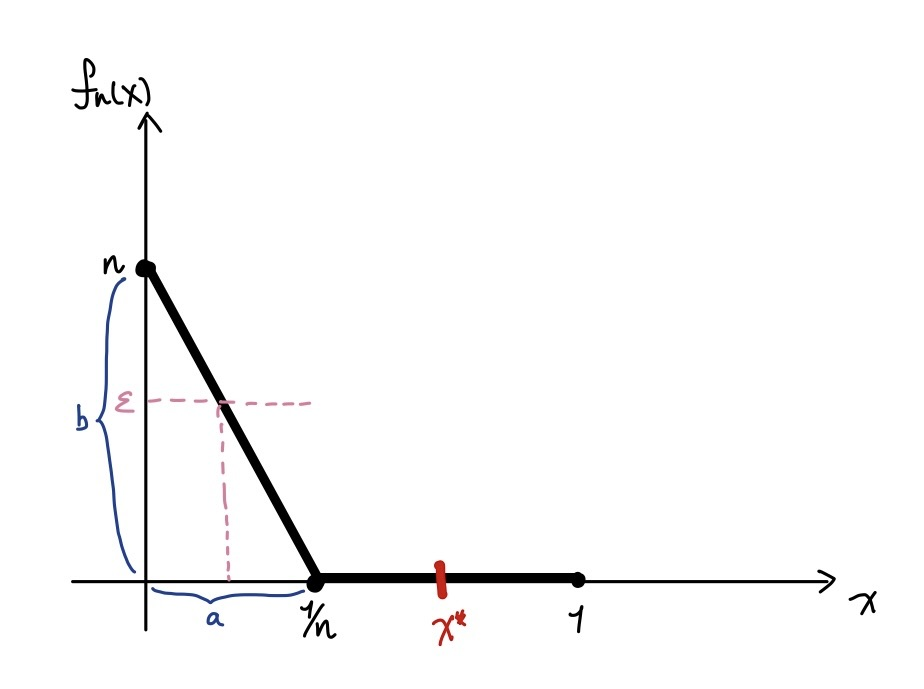
\includegraphics[scale=0.2]{Images/1.jpg} As $n\to\infty$, a becomes smaller, b becomes bigger.\\

    \begin{itemize}
        \item Point wise convergence\\
                $\forall x\in [0,1]$\\
                $\forall x^* > 0, f_n(x^*)=0\quad\text{for } n>N\quad\text{except } f_n(0)=0 \to\infty$\\

                $\Rightarrow \displaystyle f_n(x)\to
                \begin{cases}
                    0 & \text{if }x\in[0,1]\\
                    \infty & \text{if }x=0
                \end{cases} 
                \Rightarrow$ $f_n$ is not converging pointwise to the null function.
        \item Uniform convergence\\
                max $|f_n(x)| = n\, \rightarrow +\infty\quad x\in [0,1] \Rightarrow$ $f_n$ does not converge uniformly to the null function.
        \item Convergence in $L^1$
                $\rightarrow P = 1$\\
                $\displaystyle \int_{0}^{1}|f_n(x)|\, dx = \frac{1}{2} = \underbrace{\frac{1}{n}\times n\times\frac{1}{2}}_{\text{area under the triangle}}\Rightarrow$
                $f_n$ does not converge in $L^1$ to the null function.
        \item Convergence in measure\\
                $A_{n,\epsilon}\subset [0,\frac{1}{n}]$\\
                $\mu(A_{n,\epsilon})\leq\mu([0,\frac{1}{n}]) = \frac{1}{n}
                \rightarrow\text{as }n\to\infty, \mu\to\infty \Rightarrow$
                $f_n$ converges to the null function in measure.
    \end{itemize}
}

\subsection{Convergence of random variables}

Let $\{X_n\}_{n=1}^{\infty}$ be a sequence of random variables and $X$ is a random variable,
all defined in the same probability space $(\Omega, \mcA, P)$.

\dfn[]{Almost surely convergence}{
    $X_n$ converges to $X$ almost surely, or with probability 1, $X_n\xrightarrow{\text{a.s.}} X$,
    iff
    \begin{equation*}
        P[\{\omega\in\Omega : X_n(\omega)\to X(\omega)\}] = 1
    \end{equation*}
}
Similar to pointwise convergence, no need for expectation.
\nt{
    $\underbrace{P(\underbrace{X_n(\omega)}_{\text{set}}\to \underbrace{x(\omega)}_{\text{point}})}_{\text{set of which it happens has a probability of 1}} = 1$
}

\dfn[]{Convergence in the $r$th mean}{
    $X_n$ converges to $X$ in the $r$th mean, $r \geq 1$, $X_n\xrightarrow{r}X$, iff
    \begin{equation*}
        E[|X_n - X|^r]\to 0
    \end{equation*}
}
Each point will be weighted with the same probability. Expectation is involved in this case.
\nt{
    When $r = 2$, it is the mean square convergence, often used for quality checking.
}

\dfn[]{Convergence in probability}{
    $X_n$ converges in probability to $X$, $X_n\xrightarrow{P} X$, iff for all $\epsilon > 0$
    \begin{equation*}
        P(|X_n - X| > \epsilon)\to 0
    \end{equation*}
}
It is similar to measure in convergence. Often used to check for quality of estimator.
Note that this is no longer a Lebesque measure, it is now a probability measure. 
$P\{\omega\in\Omega : |X_n(\omega)-X(\omega)|>\epsilon\}\to 0$ as $n\to 0$.

\dfn[]{Convergence in distribution}{
    $X_n$ converges in distribution to $X$, $X_n\xrightarrow{d} X$, iff
    \begin{equation*}
        F_n(x)\to F_n
    \end{equation*}
    for all $x$ continuity point of F, where $F(x) = P(X\leq x)$ and $F_n(x) = P(X_n\leq x)$
}
Has nothing to do with the random variable. Often used for hypothesis testing.
It does not need the requirement that all points are defined in the same probability space $(\Omega, \mcA, P)$
as there is no $\omega$ in the density function.\\

Some useful \textbf{remarks}:
\begin{itemize}
    \item Convergence in distribution is really about the convergence of the sequence of probability functions and not the random variables themselves.
    \item When defining convergence in the $r$th mean, it is assumed that the corresponding expected values exist:\\
    $E[|X_n|^r]<\infty$ and $E[|X|^r]<\infty$
    \item When $X_n\xrightarrow{1}X$, we say that $X_n$ converges to $X$ in mean;
    when $X_n\xrightarrow{2}X$, we say that $X_n$ converges to $X$ in quadratic mean.
\end{itemize}

\begin{center}
    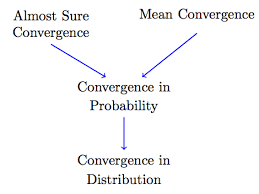
\includegraphics[scale=0.5]{Images/2.png}
\end{center}

\begin{proof}\textbf{Convergence in mean implies convergence in probability}\\

    $E[|X_n-X|]\to 0 \Rightarrow P(|X_n-X|>\epsilon)\to 0, \forall\epsilon>0$\\

    Using \textbf{Markov inequality}: $\displaystyle P(|y|>a)\leq \frac{|E[X_n-X|]}{\epsilon}$\\

    $\displaystyle 0 \leq \lim_{n\to\infty}P(|X_n-X|>\epsilon)\leq \lim_{n\to\infty}\frac{\overbrace{E[|X_n-X|]}^{\to 0}}{\epsilon}=0$
\end{proof}

\begin{proof}\textbf{Proof of convergence in probability implies convergence in distribution}\\
    
    $X_n\xrightarrow{P}X\Rightarrow X_n\xrightarrow{d} \Leftrightarrow P(|X_n-X|>\epsilon)\to 0 \Rightarrow P(X_n\leq x)\to P(X\leq x)\, ,\forall x$\\

    let $\epsilon>0$,\\

    $F_n(x)=P(X_n\leq x)$\\

    $F(x)=P(X\leq x)$\\

    Using the \textbf{total probability theorem}: $P(A) = P(A\cap B)+P(A\cap\bar{B}) = P(A|B)P(B)+P(A|\bar{B})P(\bar{B})$\\

    $F_n(x) = P(\underbrace{X_n\leq x}_{A}) 
    = P(\underbrace{X_n\leq x}_{A}, \underbrace{X\leq x+\epsilon}_{B}) 
    + P(\underbrace{X_n\leq x}_{A}, \underbrace{X>x+\epsilon}_{\bar{B}}) 
    \leq F(x+\epsilon) * P(|X_n-x|>\epsilon)$\\

    $F(x-\epsilon)-P(|X_n-X|>\epsilon)\leq F_n(x)\leq F(x+\epsilon)+\underbrace{P(|X_n-X|<\epsilon)}_{\to 0}$\\

    as $n\to\infty$, $\displaystyle \underbrace{F(x-\epsilon)}_{\xrightarrow{\epsilon\to 0} F(X)}\leq \lim_{n\to\infty}F_n(x)\leq \underbrace{F(x+\epsilon)}_{\xrightarrow{\epsilon\to 0} F(X)}$
\end{proof}

Some \textbf{converses}:
\begin{itemize}
    \item If $X_n\xrightarrow{P} X$, then there exists $\{n_k\}_{k=1}^{+\infty}$ such that $X_{n_k}\xrightarrow{a.s.} X$ when $k\to +\infty$
    \item If $|X_n|^r$ is uniformly integratable, then $X_n\xrightarrow{P} X\Rightarrow X_n\xrightarrow{r} X$
\end{itemize}
\thm[]{Skorokhod representation theorem}{
    If $X_n\xrightarrow{d}X$ then there exists a probability space $(\Omega', \mcA', P')$ and r.v. $\{Y_n\}$
    and $Y$, defined in $\Omega'$ such that
    \begin{itemize}
        \item $P'(Y_n\leq y)=P(X_n\leq y)$ and $P'(Y\leq y)=P(X\leq y)$ for all $y\in\bbR$.
        This means that $X_n$ and $Y_n$ are marginally equal in distribution, the same for $X$ and $Y$.
        \item $Y_n\xrightarrow{a.s.}Y$
    \end{itemize}
}


Other useful \textbf{results}:
\begin{itemize}
    \item $X_n\xrightarrow{P}c \Leftrightarrow X_n\xrightarrow{d}c$, where $c\in\bbR$
    \begin{proof}
        $X_n\xrightarrow{d}x\Rightarrow X_n\xrightarrow{P}c 
        \Leftrightarrow P(X_n\leq x) \to
        \begin{cases}
            0 & x<c\\
            1 & x<c
        \end{cases}$, not continuous at $c$\\
        $P(|X_n-c|>\epsilon)\to 0,\, \forall\epsilon>0$
        \begin{flalign*}
                P(|X_n-c|>\epsilon) & = P(X_n-c>\epsilon)+P(X_n-c<-\epsilon)\\
                & = P(X_n>\epsilon+c)+P(X_n<c-\epsilon)\\
                & = 1-P(X_n\leq \epsilon+c)+P(X_n<c-\epsilon)\\
                & \leq 1-P(X_n\leq \underbrace{\epsilon+c}_{>c})+P(X_n\leq \underbrace{c-\epsilon}_{<c})&&\\
                & \to 1-1+0 = 0
        \end{flalign*}
    \end{proof}
    \item Since $E[(X_n-\theta)^2]=\text{Var}(X_n)+(E[X_n]-\theta)^2$ if Var$(X_n)\to 0$ and $E[X_n]\to\theta$.
    We have convergence in mean square to $\theta$, and hence convergence in probability to $\theta$.
\end{itemize}

\thm[]{Continous mapping theorem}{
    Let $h: \bbR\to\bbR$ be a continuous function. Then
    \begin{itemize}
        \item $X_n\xrightarrow{a.s.}X\Rightarrow h(X_n)\xrightarrow{a.s.}h(X)$
        \item $X_n\xrightarrow{d}X\Rightarrow h(X_n)\xrightarrow{d}h(X)$
        \item $X_n\xrightarrow{P}X\Rightarrow h(X_n)\xrightarrow{P}h(X)$
    \end{itemize}
}
\thm[]{Slutsky theorem}{
    Let $\{X_n\}$ and $\{Y_n\}$ be sequences of random variables, $X$ a random variable and c a real number.
    If $X_n\xrightarrow{d}X$ and $Y_n\xrightarrow{p}c$, then
    \begin{itemize}
        \item $X_n + Y_n\xrightarrow{d}X+c$
        \item $Y_n\,X_n\xrightarrow{d}cX$
        \item $X_n/Y_n\xrightarrow{d}X/c$ as long as $c\neq 0$
    \end{itemize}
}
\wc[]{$X_n+Z_n\neq 2X$}{
    Suppose that $X_n\xrightarrow{d}X$ where $X\sim N(0,1)$. Then with $Z_n = -X_n$ we have $Z_n\xrightarrow{d}X$.
    However, $X_n + Z_n = 0$, hence $X_n + Z_n$ does not converge in distribution to $2X$ as one might expect.\\

    cdf of $Z_n$ converges to cdf of $X_n$
    \begin{flalign*}
    Z_n\xrightarrow{d}X & \Leftrightarrow P(Z_n\leq z_n)\to\Phi(z_n),\, \forall z\in\bbR\\
    & \Leftrightarrow P(-X_n\leq z) = P(X_n\geq -z) = 1-P(X_n\leq -z)\\
    & \rightarrow 1-\Phi(-z)\\
    \therefore Z_n\xrightarrow{d}X
    \end{flalign*}
    This is why the Slutsky theorem is important, it showcases safe procedures.
}
\ex[]{$X_n\sim t(n)\Rightarrow X_n\xrightarrow{d}N(0,1)$ using Slutsky}{
    $X_n\sim t(n)$, $\displaystyle X_n = \frac{u_n}{\sqrt{\frac{v_n}{n}}}$\\

    Assumptions:
    $\begin{cases}
        u_n\text{independent of }v_n\\
        u_n\sim N(0,1)\\
        v_n\sim \chi^2(n)
    \end{cases}$

    What would be nice is to show that $\sqrt{\frac{v_n}{n}}$ converges to 1 then we can apply the Slutsky theorem.\\

    Using the \textbf{mean square convergence}, we have
    \begin{align*}
        \text{Var}(\frac{v_n}{n}) & = \frac{\text{Var}(v_n)}{n} = \frac{2n}{n^2} = \frac{2}{n}\rightarrow 0\\
        E[\frac{v_n}{n}] & = \frac{E[v_n]}{n} = \frac{n}{n} = 1 \rightarrow 1
    \end{align*}
    We now have mean square convergence to 1.\\

    Using the \textbf{Continuous mapping theorem}, we have
    \begin{equation*}
        \frac{v_n}{n}\xrightarrow{P}1 \Rightarrow \sqrt{\frac{v_n}{n}}\xrightarrow{P}1 
    \end{equation*}

    $\Rightarrow \displaystyle \frac{v_n}{n}\xrightarrow{2}1$ and $\displaystyle\frac{v_n}{n}\xrightarrow{P}1$\\

    Now using the \textbf{Slutsky theorem}, we have
    \begin{equation*}
        X_n = \frac{u_n}{\sqrt{\frac{v_n}{n}}}\xrightarrow{d}u_n\sim N(0,1)
    \end{equation*}
}

\section{Important asymptotic results}

\thm[]{Weak law of large numbers}{
    Let $\{X_n\}_{n=1}^{+\infty}$ be a sequence of independent and identically distributed random variables,
    with $E[X_n]=\mu$ and Var$(X_n)=\sigma^2<\infty$. Let also $\overline{X}_n = \frac{1}{n}\sum_{i=1}^{n}X_i$.
    Then we have that
    \begin{equation*}
        \overline{X}_n\xrightarrow{P}\mu
    \end{equation*}
}
\begin{proof}
    Goal: $\overline{X}_n\xrightarrow{P}\mu\Rightarrow P(|\overline{X}_n-\mu|>\epsilon)\to 0$\\

    Checking the validity of Chebychov's inequality,
    \begin{equation*}
        E[\overline{X}_n]=E[\frac{1}{n}\sum_{i=1}^{n}X_i]
        =\frac{1}{n}\sum_{i=1}^{n}\underbrace{E[X_i]}_{\to\mu} 
        =\frac{1}{n}\, n\, \mu = \mu
    \end{equation*}
    We can now apply the \textbf{Chebychov's inequality}: 
    $\displaystyle P(\underbrace{|X-\mu|}_{\text{distance of distribution from its mean}}>\epsilon)\leq\frac{\text{Var}(X)}{\epsilon^2}$\\

    $\displaystyle P(|\overline{X}_n-\mu|>\epsilon)\leq \frac{\overbrace{\text{Var}(\overline{X}_n)}^{1}}{\epsilon^2} = \frac{\sigma^2}{n\, \epsilon^2}\to 0$\\

    1: Var$\displaystyle (\overline{X}_n) = \frac{1}{n}\text{Var}(\sum_{i=1}^{n}X_i) \underbrace{=}_{\text{Var}(\sum)=\sum\text{Var}+\underbrace{2\text{Cov}}_{\text{iid}\to 0}} \frac{1}{n^2}\, n\, \sigma^2 = \frac{\sigma^2}{n}$
\end{proof}

Intuitively, the WLLN tell us that $\overline{X}_n$ becomes more and more concentrated around $\mu$ as $n$ increases.

\thm[]{Strong law of large numbers}{
    Under the same conditions as above, we have\\
    \begin{equation*}
        \overline{X}_n\xrightarrow{a.s.}\mu
    \end{equation*}
}

Actually, it is only necessary to assume that $E[|X_i|]<+\infty$ for both laws to hold.

\thm[]{Central limit theorem}{
    Let $\{X_n\}_{n=1}^{+\infty}$ be a sequence of iid random variables possessing finite variance.
    Let $\mu = E[X_n]$ and $\sigma^2 = \text{Var}(X_n)$.
    Let also $\overline{X}_n = \frac{1}{n}\sum_{i=1}^{n}X_i$ and
    \begin{equation*}
        Z_n = \sqrt{n}\,\frac{\overline{X}_n-\mu}{\sigma} = \frac{\overline{X}_n-\mu}{\sqrt{\frac{\sigma^2}{n}}}=\frac{\overline{X}_n-E[\overline{X}]}{\sqrt{\text{Var}(\overline{X})}}\xrightarrow{d}N(0,1)
    \end{equation*}
    Then we have
    \begin{equation*}
        Z_n\xrightarrow{d}Z
    \end{equation*}
    where $Z\sim N(0,1)$
}

\begin{proof}
    \textbf{Proof with assumption of existance of mgf}\\

    \noindent 
    Assume 
    \begin{enumerate}
        \item $M_n(S) = E[e^{sX_n}]$ exists
        \item $M_n(s)\to M(s)$ for $s\in(-s_0,s_0)$
    \end{enumerate}
    then $M(s) = E[e^{sX}]\Rightarrow X_n\xrightarrow{d}X$\\

    \noindent
    Idea: $X_n$ are iid r.v.\\
    $E[e^{sX_n}] = M_{X_n}(s)$ exists for $s\in(-s_0,s_0) \Rightarrow Z_n = \sqrt{n}\frac{\bar{X}_n-\mu}{\sigma}$\\
    Need to show $M_{Z_n}(s)\to M_{N(0,1)}(s) = e^{s^2/2}\rightarrow$ mgf of $Z_n$ goes to $e^{s^2/2}$, the mgf of the normal distribution.
    \begin{equation}
        Z_n = \sqrt{n}\frac{\overline{X}_n-\mu}{\sigma}\underbrace{=}_{\text{Annex 1}}\frac{1}{\sqrt{n}}\sum_{i=1}^{n}y_i
    \end{equation}
Annex 1: 
\begin{equation*}
\begin{split}
    Y_i & = \frac{X_i-\mu}{\sigma}, \text{standardized version of the $X_i$'s}\\
    \sum Y_i & = \frac{\sum (X_i-\mu)}{\sigma} = \frac{\sum X_i - n\mu}{\sigma} = \frac{n\overline{X}_n-n\mu}{\sigma} = n\frac{\overline{X}_n-mu}{\sigma}\\
    \frac{1}{\sqrt{n}}\sum Y_i & = \frac{1}{\sqrt{n}}n\frac{\overline{X}_n-mu}{\sigma}=\sqrt{n}\frac{\overline{X}_n-\mu}{\sigma}
\end{split}
\end{equation*}

Using the moment generating function
\begin{equation}
    \begin{split}
        M_{Z_n}(s) & = E[e^{sZ_n}] = E[e^{s\frac{1}{\sqrt{n}}\sum Y_i}]\\
        & =M_{\sum Y_i}(\frac{s}{\sqrt{n}})\\
        & =M_{Y_1}(\frac{s}{\sqrt{n}})\times M_{Y_2}(\frac{s}{\sqrt{n}})\times \cdots \times M_{Y_n}(\frac{s}{\sqrt{n}})\rightarrow\text{mgf of the sum of the variable is the product}\\
        & = [M_Y(\frac{s}{\sqrt{n}})]^n\\
        & = \sum_{k=0}^{2}M_Y^{(k)}(0)\frac{s^k}{k!}+\underbrace{r(s)}_{\frac{r(s)}{s^2}\to 0 \text{ as }s\to 0} \rightarrow\text{Taylor's expansion of 2nd order, Annex 2}\\
        & = 1 + \frac{s^2}{2!}+r(s)       
    \end{split}
\end{equation}

Annex 2:
\begin{equation*}
    \begin{split}
        M_Y^{(k)}(0) & = E[Y^k]\\
        M_Y^{(0)}(0) & = E[Y^0] = 1\\
        M_Y^{(1)}(0) & = E[Y^1] = 0\\
        M_Y^{(2)}(0) & = E[Y^2] = \frac{E[(x_i-\mu)^2]}{\sigma^2} = \frac{\sigma^2}{\sigma^2} = 1
    \end{split}
\end{equation*}

Back to the moment generating function
\begin{equation}
    \begin{split}
        M_{Z_n}(s) & = [M_Y(\frac{s}{\sqrt{n}})]^n\\
        & = [1 + \frac{s^2/2}{n} + r(\frac{s}{\sqrt{n}})]^n\\
        & = [1 + \frac{\frac{s^2}{2} + n\overbrace{r(s/\sqrt{n})}^{\to 0}}{n}]^n \underbrace{\rightarrow}_{\text{Annex 3}} e^{s^2/2}
    \end{split}
\end{equation}

Annex 3:
\begin{equation*}
    [1 + \frac{u_n}{v_n}]^{v_n}\to e^c, u_n\to c, v_n \to \infty
\end{equation*}
\end{proof}

The CLT is often used to compute probabilities of the type $P(\overline{X}_n\leq x)$ approximating them by $\Phi(\sqrt{n}\frac{(x-\mu)}{\sigma})$ for sufficiently large $n$.
\begin{flalign*}
    P(\overline{X}_n\leq x) & =P(\sqrt{n}\frac{\bar{X}-\mu}{\sigma}\leq \sqrt{n}\frac{x-\mu}{\sigma})\\
    & \approx \Phi(\sqrt{n}\frac{x-\mu}{\sigma})\\
    P(Z_n\leq z) & \rightarrow \Phi(z)
\end{flalign*}
Intuitively, the CLT tells us that the distribution of $\bar{X}_n$ is well approximated by a normal distribution for sufficiently large $n$ 
as long as the variance is finite.
Additionally, if the distribution of $X_n$ is close to symmetric, then the rate of convergence is faster.
Rate of convergence is related to the coefficient of symmetry, $\displaystyle\frac{E[(X-\mu)^3]}{(\text{Var}(X))^{3/2}}=\gamma_1$.
If the distribution is symmetric, $\gamma_1=0$.

\thm[]{Lévy's continuity theorem}{
    Suppose that $\{X_n\}_{n=1}^{+\infty}$ is a sequence of random variables and let $M_n(s)$ denote the mgf of $X_n, n=1,2,\cdots$.\\
    Additionally assume that
    \begin{equation*}
        \lim_{n\to +\infty}M_n(s) = M(s)
    \end{equation*}
    for $s$ in a neighborhood of the origin, and that $M(\cdot)$ is the mgf of a random variable $X$.\\

    In these circumstances, 
    \begin{equation*}
        X_n\xrightarrow{d}X
    \end{equation*}
}

\ex[]{Application : Bernoulli}{
    $\{X_n\}_{n=1}^{+\infty}$ iid $B(1,\theta)$ where $\theta\in (0,1)$. By the \textbf{central limit theorem},
    \begin{equation*}
        \sqrt{n}\frac{\overline{X}_n-\theta}{\sqrt{\theta(1-\theta)}}\xrightarrow{d}N(0,1)
    \end{equation*}
    On the other hand, the \textbf{WLLN} ensures that $\overline{X}_n\xrightarrow{d}\theta$.\\
    By the \textbf{continuous mapping theorem},
    \begin{equation*}
        \frac{\sqrt{\theta(1-\theta)}}{\sqrt{\overline{X}_n(1-\overline{X}_n)}}\xrightarrow{P}1
    \end{equation*}
    and \textbf{Slutsky's theorem} allows us to conclude that
    \begin{equation*}
        \sqrt{n}\,\frac{\overline{X}_n-\theta}{\sqrt{\theta(1-\theta)}}\, \frac{\sqrt{\theta(1-\theta)}}{\sqrt{\overline{X}_n(1-\overline{X}_n)}} = \sqrt{n}\,\frac{\overline{X}_n-\theta}{\sqrt{\overline{X}_n(1-\overline{X}_n)}}\xrightarrow{d}N(1,0)
    \end{equation*}
    which in practice means that, for large $n$
    \begin{equation*}
        P\left(\frac{\overline{X}_n-\theta}{\sqrt{\overline{X}_n(1-\overline{X}_n)}}\leq x\right)\approx \Phi(x)
    \end{equation*}
}
\begin{proof}
    $X_i\sim B(1,\theta), \quad E[x_i]=\theta\quad \text{Var}(x_i)=\theta(1-\theta)$\\

    By the \textbf{CLT},
    $\displaystyle \sqrt{n}\, \frac{\overline{X}_n-\theta}{\underbrace{\sqrt{\theta(1-\theta)}}_{\text{issue in the denominator}}}\xrightarrow{d}N(0,1)$\\

    $\displaystyle \sqrt{n}\, \frac{\overline{X}_n-\theta}{\sqrt{\overline{X}_n(1-\overline{X}_n)}}\xrightarrow{d}N(0,1)
    = \underbrace{\sqrt{n}\, \frac{\overline{X}_n-\theta}{\sqrt{\theta(1-\theta)}}}_{\xrightarrow{d}N(0,1)\text{ by CLT}}\, \underbrace{\frac{\sqrt{\theta(1-\theta)}}{\sqrt{\overline{X}_n(1-\overline{X}_n)}}}_{\xrightarrow{P}1\text{, Annex 1}}$\\

    Annex 1:
    \begin{itemize}
        \item $\overline{X}_n\xrightarrow{P}E[X_i]=\theta\text{ by \textbf{WLLN}}$
        \item $\sqrt{\overline{X}_n(1-\overline{X}_n)}\to \sqrt{\theta(1-\theta)}\text{ by \textbf{continuous mapping theorem}}$
    \end{itemize}
\end{proof}

\ex[]{Application : $P(X\in A)$ using Simple Monte Carlo}{
    Notice that $P(X\in A)=E[Y]$ where $Y = I_A(X) = \begin{cases}
        1 & ,x\in A\\
        0 & ,x\not\in A
    \end{cases}$\\

    Let $X_1, X_2,\cdots, X_M$ be iid r.v. with the same distribution as $X$, and $Y_i=I_A(X_i), i=1,\ldots,M$.
    Then by \textbf{SLLN},
    \begin{equation*}
        \bar{Y}_M = \frac{1}{M}\sum_{i=1}^{M}Y_i\xrightarrow{a.s.}E[Y] = P(X\in A)
    \end{equation*}
    where $M$ is the simulation length.\\

    For sufficiently large M,
    \begin{equation*}
        P(X\in A)\approx \frac{1}{M}\sum_{i=1}^{M}y_i = \frac{1}{M}\underbrace{\#\{i=1,\ldots,M : x_i\in A}_{\text{observed proportions of }x_i\in A}\}
    \end{equation*}
}

Simple Monte Carlo allows us to replace the analytical knowledge of a probability distribution by a sufficiently large sample of iid draws from the distribution 
since almost all aspects of that probability distribution can be arbitrarilly approximated using that sample.

\ex[]{Application : $f(a)$ for some $a\in\bbR$ using Simple Monte Carlo}{
    For a continous distribution with density $f$,
    \begin{equation*}
        \begin{split}
            f(a) & = \lim_{\delta\to 0}\frac{F(a+\delta-F(a))}{\delta}\\
            & = \frac{1}{\delta}\, \frac{1}{M}\#\{i=1,\ldots,M : a<x_i<a+\delta\}
        \end{split}
    \end{equation*}
    That is, the histogram of $x_1,\ldots,x_M$ is an approximation to the density of $X$.
}

\thm[]{Delta method}{
    Let $\{X_n\}_{n=1}^{+\infty}$ be a sequence of r.v. such that $\forall\theta\in\Theta$
    \begin{equation*}
        \sqrt{n}(X_n-\theta)\xrightarrow{d}N(0,\sigma^2)
    \end{equation*}
    Let $\underbrace{\theta_0}_{\text{interior point of }\Theta}\in\overbrace{\Theta}^{\text{open set}}$ and $g$ be a differentiable function such that
    $g'(\theta_0)\neq 0$. Then
    \begin{equation*}
        \sqrt{n}(\underbrace{g(X_n)}_{\text{typically non-linear}}-g(\theta_0))\xrightarrow{d}N(0, \sigma^2[g'(\theta_0)]^2)
    \end{equation*}
}
\begin{proof}
    Using the 1st order Taylor expansion\\
    $\displaystyle g(x) = g(\theta_0) + g'(\theta_0)(x-\theta_0)+r(x-\theta_0),\quad \frac{r(x-\theta_0)}{x-\theta_0}\to 0 \text{ as }x\to\theta_0$
    \begin{flalign*}
        g(x_n)-g(\theta_0) & = g'(\theta_0)(x_n-\theta_0) + r(x_n-\theta_0)\\
        \sqrt{n}\,(g(x_n)-g(\theta_0)) & = \underbrace{\sqrt{n}\,(g(x_n)-g(\theta_0))}_{\text{Annex 1}} + \underbrace{\sqrt{n}\,r(x_n-\theta_0)}_{\text{Annex 2}}\\
        \sqrt{n}\,(g(x_n)-g(\theta_0)) & = \underbrace{\sqrt{n}\,(g(x_n)-g(\theta_0))}_{\xrightarrow{d}N(0,[g'(\theta_0)]^2\sigma^2)} + \underbrace{\sqrt{n}\,r(x_n-\theta_0)}_{\xrightarrow{P} 0}
    \end{flalign*}
    Annex 1:\\
    $\sqrt{n}(x_n-\theta_0)\xrightarrow{d}N(0,\sigma^2)$\\
    By \textbf{Slutsky's theorem}, $\underbrace{g'(\theta_o)}_{\text{constant, }\xrightarrow{P}g'(\theta_0)}\underbrace{\sqrt{n}(x_n-\theta_0)}_{\xrightarrow{d}T(\cdot)}
    \xrightarrow{d}g'(\theta_0)N(0,\sigma^2) = N(0\times g'(\theta_0), [g'(\theta_0)]^2\sigma^2)$ \\
    $\Rightarrow \sqrt{n}(x_n-\theta_0)\xrightarrow{d}N(0,[g'(\theta_0)]^2\sigma^2)$\bigskip\\
    Annex 2:\\
    Step 1:\\
    $\displaystyle(T_n-\theta) = \underbrace{\frac{1}{a_n}}_{\xrightarrow{P}0}\, \underbrace{a_n(T_n-\theta)}_{\xrightarrow{d}T(\cdot)}\xrightarrow{d}0\times T(\cdot) = 0
    \Rightarrow T_n\xrightarrow{d}\theta \underbrace{\Leftrightarrow}_{\text{this applies because $\theta$ is a constant}} T_n\xrightarrow{P}\theta$\\
    $\therefore \sqrt{n}(T_n-\theta)\xrightarrow{d}T\Rightarrow T_n\xrightarrow{P}\theta$\\
    Step 2:\\
    $\sqrt{n}(x_n-\theta_0)\xrightarrow{d}N(0,\sigma^2)$\\
    By step 1, we can conclude that $x_n\xrightarrow{P}\theta_0\quad X_n-\theta_0\xrightarrow{P}0$\\
    We also know that $\displaystyle\frac{r(x)}{x}\to 0$\\
    By \textbf{continuous mapping theorem}, $\displaystyle \frac{r(x_n-\theta_0)}{x_n-\theta_0}\xrightarrow{P}0$\\
    Step 3:\\
    $\displaystyle\sqrt{n}\, r(x_n-\theta_0) \Leftrightarrow \underbrace{\sqrt{n}(x_n-\theta_0)}_{\xrightarrow{d}N(0,\sigma^2)}\underbrace{\frac{r(x_n-\theta_0)}{x_n-\theta_0}}_{\xrightarrow{P}0}$\\
    By \textbf{Slutsky's theorem}, 
    $\displaystyle\sqrt{n}\,r(x_n-\theta_0)\xrightarrow{d}0\underbrace{\Rightarrow}_{\text{true for constant}}\sqrt{n}r(x_n-\theta_0)\xrightarrow{P}0$
\end{proof}

\ex[]{Application : log-odds ratio}{
    Suppose that $X_1,\ldots,X_n$ are iid $B(1,\theta)$. Then the \textbf{CLT} ensures that
    \begin{equation*}
        \sqrt{n}\frac{\bar{X}_n-\theta}{\sqrt{\theta(1-\theta)}}\xrightarrow{d}N(0,1)
    \end{equation*}
    which is equivalent to $\sqrt{n}(\bar{X}_n-\theta)\xrightarrow{d}N(0,\theta(1-\theta))$.
    \begin{itemize}
        \item $\bar{X}_n=\frac{1}{n}\sum_{i=1}^{n}x_i$ representing the proportion of successes in the random sample
        \item $\theta$ representing the probability of success in the population
    \end{itemize}
    Now we are interested in the asymptotic distrbution of $Y_n=\ln\frac{\bar{X}_n}{1-X_n}$ which is the empirical log odds of success, a non-linear function.
    With $g(x) = \ln\frac{x}{1-x}$, following $g'(x) = \frac{1}{x(1-x)}$. The \textbf{delta method} ensures that
    \begin{equation*}
        \sqrt{n}(Y_n - \ln\frac{\theta}{1-\theta})\xrightarrow{d} N(0, [\theta(1-\theta)]^{-1})
    \end{equation*}
    which is often written as
    \begin{equation*}
        Y_n\overset{a}{\sim} N(\ln\frac{\theta}{1-\theta}, \frac{[\theta(1-\theta)]^{-1}}{n})
    \end{equation*}
}
\begin{proof}
    Asymptotic distribution of $T_n = \ln\frac{\bar{X}_n}{1-\bar{X}_n}$\bigskip\\
    $\sqrt{n}\frac{\bar{X}_n-\theta}{\sqrt{\theta(1-\theta)}}\xrightarrow{d} N(0,1) \Leftrightarrow \sqrt{n}(\bar{X}_n-\theta)\xrightarrow{d} N(0, \theta(1-\theta))$\\
    $\displaystyle g(x) = \ln\frac{x}{1-x} \rightarrow g'(x)=\frac{(\frac{x}{1-x})}{(\frac{x}{1-x})} = \frac{\frac{1-x-(-1)x}{(1-x)^2}}{\frac{x}{1-x}} = \frac{1-x+x}{(1-x)^2}\,\frac{1-x}{x} = \frac{1}{x(1-x)}$\bigskip\\
    Applying the \textbf{delta method}, $\sqrt{n}(T_n-g(\theta_0))\xrightarrow{d} N(0, [g'(\theta_0)]^2\sigma^2)$\bigskip\\
    $\displaystyle \Rightarrow \sqrt{n}(T_n - \ln\frac{\theta_0}{1-\theta_0})\xrightarrow{d} N\left(0, \left(\frac{1}{\theta(1-\theta)}\right)^2\theta_0(1-\theta_0)\right)
    \Leftrightarrow \sqrt{n}(T_n - \ln\frac{\theta_0}{1-\theta_0})\xrightarrow{d} N(0, [\theta_0(1-\theta_0)]^{-1})$
\end{proof}

\ex[]{Application : variance stabalizing}{
    Suppose $X_1,\ldots,X_n$ are $B(0,\theta)$. Then the \textbf{CLT} ensures that
    \begin{equation*}
        \sqrt{n}\frac{\bar{X}_n-\theta}{\sqrt{\theta(1-\theta)}}\xrightarrow{d}N(0,1)
    \end{equation*}
    Note that the asymptotic variance depends on the true value of $\theta$, meaning that the variance, $\sigma^2$ is not fixed, thus giving us the motive to stabalize the variance.
    Our goal is to find a $g$ such that $\sqrt{n}(g(\bar{X}_n)-g(\theta))\xrightarrow{d} N(0,1)$, which is the same as solving for $g'(x) = \frac{1}{\sqrt{\theta(1-\theta)}}$.\bigskip\\
    $[g'(x)]^2\theta(1-\theta) = 1 \Leftrightarrow g'(x) = \frac{1}{\theta(1-\theta)} = \theta^{-1/2}(1-\theta)^{-1/2} \Rightarrow g(\theta)=2\,\arcsin\sqrt{\theta}$\\

    After this, the asymptotic distribution would be normal with a constant variance.
    \begin{equation*}
        \sqrt{n}(2\,\arcsin\sqrt{\bar{X}_n}-2\,\arcsin\sqrt{\theta})\xrightarrow{d} N(0,1)
    \end{equation*}
    
    When can we apply this technique?\\
    $\sqrt{n}(X_n-\mu)\xrightarrow{d} N(0, \ln(\mu))$\\
    From \textbf{delta method}, $\sqrt{n}(g(X_n)-g(\mu))\xrightarrow{d}N(0, [g'(\mu)]^2 ln(\mu))$\\
    the variance stabalizing transformation $g$ satisfies $\displaystyle [g'(x)]^2 \ln(\mu) = 1 \Leftrightarrow g'(\mu) = \frac{1}{\sqrt{\ln(\mu)}} \Rightarrow g(\mu)=\int_{c}^{\mu}\frac{1}{h(t)}\, dt$\\
    $c$ being some constant that ensures the integral exists, and with this $c$,\\
    $\sqrt{n}(g(x_n)-g(\mu))\xrightarrow{d} N(0,1)$
}